\section{C/C++ Sample applications}
\label{sec:CSampleApps}

The first two examples in this section are simple applications developed in COMPSs to easily illustrate how to code,
compile and run COMPSs applications. These applications are executed locally and show different ways to take advantage
of all the COMPSs features. 

The rest of the examples are more elaborated and consider the execution in a cloud platform where the VMs mount a common 
storage on \textbf{/sharedDisk} directory. This is useful in the case of applications that require working 
with big files, allowing to transfer data only once, at the beginning of the execution, and to enable 
the application to access the data directly during the rest of the execution.

The Virtual Machine available at our webpage (\url{http://compss.bsc.es/}) provides a development environment with
all the applications listed in the following sections. The codes of all the applications can be found under the 
$/home/compss/workspace\_c/$ folder. 


%%%%%%%%%%%%%%%
%% SIMPLE
%%%%%%%%%%%%%%%
\subsection{Simple}
The Simple application is a C application that increases a counter by means of a task. The counter is stored inside a file that 
is transfered to the worker when the task is executed. Thus, the tasks inferface is defined as follows:

\begin{lstlisting}[language=c]
  // simple.idl
  interface simple {
	  void increment(inout File filename);
  };
\end{lstlisting}

Next we also provide the invocation of the task from the main code and the increment's method code.

\begin{lstlisting}[language=c]
  // simple.cc
	
  int main(int argc, char *argv[]) {
      // Check and get parameters
      if (argc != 2) {
	  usage();
	  return -1;
      }
      string initialValue = argv[1];
      file fileName = strdup(FILE_NAME);

      // Init compss
      compss_on();

      // Write file
      ofstream fos (fileName);
      if (fos.is_open()) {
	  fos << initialValue << endl;
	  fos.close();
      } else {
	  cerr << "[ERROR] Unable to open file" << endl;
	  return -1;
      }
      cout << "Initial counter value is " << initialValue << endl;

      // Execute increment
      increment(&fileName);
      compss_wait_on(fileName);

      // Read new value
      string finalValue;
      ifstream fis (fileName);
      if (fis.is_open()) {
	  if (getline(fis, finalValue)) {
	      cout << "Final counter value is " << finalValue << endl;
	      fis.close();
	  } else {
	      cerr << "[ERROR] Unable to read final value" << endl;
	      fis.close();
	      return -1;
	  }
      } else {
	  cerr << "[ERROR] Unable to open file" << endl;
	  return -1;
      }

      // Close COMPSs and end
      compss_off();
      return 0;
  }
\end{lstlisting}

\begin{lstlisting}[language=c]
  //simple-functions.cc
  
  void increment(file *fileName) {
      cout << "INIT TASK" << endl;
      cout << "Param: " << *fileName << endl;
      // Read value
      char initialValue;
      ifstream fis (*fileName);
      if (fis.is_open()) {
	  if (fis >> initialValue) {
	      fis.close();
	  } else {
	      cerr << "[ERROR] Unable to read final value" << endl;
	      fis.close();
	  }
	  fis.close();
      } else {
	  cerr << "[ERROR] Unable to open file" << endl;
      }

      // Increment
      cout << "INIT VALUE: " << initialValue << endl;
      int finalValue = ((int)(initialValue) - (int)('0')) + 1;
      cout << "FINAL VALUE: " << finalValue << endl;

      // Write new value
      ofstream fos (*fileName);
      if (fos.is_open()) {
	  fos << finalValue << endl;
	  fos.close();
      } else {
	  cerr << "[ERROR] Unable to open file" << endl;
      }
      cout << "END TASK" << endl;
  }
\end{lstlisting}

Finally, to compile and execute this application users must run the following commands:

\begin{lstlisting}[language=bash]
compss@bsc:~$ cd ~/workspace_c/simple/
compss@bsc:~/workspace_c/simple$ buildapp simple
compss@bsc:~/workspace_c/simple$ runcompss --lang=c --project=./xml/project.xml --resources=./xml/resources.xml ~/workspace_c/simple/master/simple 1

----------------- Executing simple --------------------------

JVM_OPTION_FILE: /tmp/tmp.X3MVgWY1L1 
IT_HOME: /opt/COMPSs//Runtime/scripts/user/../.. 
Args: 1 

WARNING: IT Properties file is null. Setting default values
[   API]  -  Starting COMPSs Runtime v1.3 (build 20151030-0946.rnull)
Initial counter value is 1
[   BINDING]  -  @GS_register  -  Ref: 0x7ffe027514c8
[   BINDING]  -  @GS_register  -  ENTRY ADDED
[   BINDING]  -  @GS_register  -  Entry.type: 0
[   BINDING]  -  @GS_register  -  Entry.classname: File
[   BINDING]  -  @GS_register  -  Entry.filename: counter
[   BINDING]  -  @compss_wait_on  -  Entry.type: 0
[   BINDING]  -  @compss_wait_on  -  Entry.classname: File
[   BINDING]  -  @compss_wait_on  -  Entry.filename: counter
[   BINDING]  -  @compss_wait_on  -  Runtime filename: /home/compss/.COMPSs/simple_01/tmpFiles/d1v2_1446817611279.IT
[   BINDING]  -  @compss_wait_on  -  File renaming: /home/compss/.COMPSs/simple_01/tmpFiles/d1v2_1446817611279.IT to counter
Final counter value is 2
[   API]  -  No more tasks for app 0
[   API]  -  Getting Result Files 0
[   API]  -  Execution Finished

------------------------------------------------------------
\end{lstlisting}


%%%%%%%%%%%%%%%
%% INCREMENT
%%%%%%%%%%%%%%%
\subsection{Increment}
The Increment application is a C application that increases N times three different counters. Each increase step is developed by a separated task. The
purpose of this application is to show parallelism between the three counters.

Next we provide the main code of this application. The code inside the \textit{increment} task is the same than the previous example. 

\begin{lstlisting}[language=c]
  // increment.cc
  
  int main(int argc, char *argv[]) {
      // Check and get parameters
      if (argc != 5) {
	  usage();
	  return -1;
      }
      int N = atoi( argv[1] );
      string counter1 = argv[2];
      string counter2 = argv[3];
      string counter3 = argv[4];

      // Init COMPSs
      compss_on();

      // Initialize counter files
      file fileName1 = strdup(FILE_NAME1);
      file fileName2 = strdup(FILE_NAME2);
      file fileName3 = strdup(FILE_NAME3);
      initializeCounters(counter1, counter2, counter3, fileName1, fileName2, fileName3);

      // Print initial counters state
      cout << "Initial counter values: " << endl;
      printCounterValues(fileName1, fileName2, fileName3);

      // Execute increment tasks
      for (int i = 0; i < N; ++i) {
	  increment(&fileName1);
	  increment(&fileName2);
	  increment(&fileName3);
      }

      // Sync master
      compss_wait_on(fileName1);
      compss_wait_on(fileName2);
      compss_wait_on(fileName3);

      // Print final state
      cout << "Final counter values: " << endl;
      printCounterValues(fileName1, fileName2, fileName3);

      // Stop COMPSs
      compss_off();

      return 0;
  }
\end{lstlisting}

As shown in the main code, this application has 4 parameters that stand for:

\begin{enumerate}
 \item \textbf{N:} Number of times to increase a counter
 \item \textbf{counter1:} Initial value for counter 1
 \item \textbf{counter2:} Initial value for counter 2
 \item \textbf{counter3:} Initial value for counter 3
\end{enumerate}

Next we will compile and run the Increment application with the \textit{-g} option to be able to generate the final graph at the end 
of the execution.

\begin{lstlisting}[language=bash]
compss@bsc:~$ cd ~/workspace_c/increment/
compss@bsc:~/workspace_c/increment$ buildapp increment
compss@bsc:~/workspace_c/increment$ runcompss --lang=c -g --project=./xml/project.xml --resources=./xml/resources.xml ~/workspace_c/increment/master/increment 10 1 2 3

----------------- Executing increment --------------------------

JVM_OPTION_FILE: /tmp/tmp.TsZ1Y3j5bM 
IT_HOME: /opt/COMPSs//Runtime/scripts/user/../.. 
Args: 10 1 2 3 

WARNING: IT Properties file is null. Setting default values
[   API]  -  Starting COMPSs Runtime v1.3 (build 20151030-0946.rnull)
Initial counter values: 
- Counter1 value is 1
- Counter2 value is 2
- Counter3 value is 3
[   BINDING]  -  @GS_register  -  Ref: 0x7ffdd12596b0
[   BINDING]  -  @GS_register  -  ENTRY ADDED
[   BINDING]  -  @GS_register  -  Entry.type: 0
[   BINDING]  -  @GS_register  -  Entry.classname: File
[   BINDING]  -  @GS_register  -  Entry.filename: file1.txt
[   BINDING]  -  @GS_register  -  Ref: 0x7ffdd12596b8
[   BINDING]  -  @GS_register  -  ENTRY ADDED
[   BINDING]  -  @GS_register  -  Entry.type: 0
[   BINDING]  -  @GS_register  -  Entry.classname: File
[   BINDING]  -  @GS_register  -  Entry.filename: file2.txt
[   BINDING]  -  @GS_register  -  Ref: 0x7ffdd12596c0
[   BINDING]  -  @GS_register  -  ENTRY ADDED
[   BINDING]  -  @GS_register  -  Entry.type: 0
[   BINDING]  -  @GS_register  -  Entry.classname: File
[   BINDING]  -  @GS_register  -  Entry.filename: file3.txt
[   BINDING]  -  @GS_register  -  Ref: 0x7ffdd12596b0
[   BINDING]  -  @GS_register  -  ENTRY FOUND
[   BINDING]  -  @GS_register  -  Entry.type: 0
[   BINDING]  -  @GS_register  -  Entry.classname: File
[   BINDING]  -  @GS_register  -  Entry.filename: file1.txt
[   BINDING]  -  @GS_register  -  Ref: 0x7ffdd12596b8
[   BINDING]  -  @GS_register  -  ENTRY FOUND
[   BINDING]  -  @GS_register  -  Entry.type: 0
[   BINDING]  -  @GS_register  -  Entry.classname: File
[   BINDING]  -  @GS_register  -  Entry.filename: file2.txt
[   BINDING]  -  @GS_register  -  Ref: 0x7ffdd12596c0
[   BINDING]  -  @GS_register  -  ENTRY FOUND
[   BINDING]  -  @GS_register  -  Entry.type: 0
[   BINDING]  -  @GS_register  -  Entry.classname: File
[   BINDING]  -  @GS_register  -  Entry.filename: file3.txt
[   BINDING]  -  @GS_register  -  Ref: 0x7ffdd12596b0
[   BINDING]  -  @GS_register  -  ENTRY FOUND
[   BINDING]  -  @GS_register  -  Entry.type: 0
[   BINDING]  -  @GS_register  -  Entry.classname: File
[   BINDING]  -  @GS_register  -  Entry.filename: file1.txt
[   BINDING]  -  @GS_register  -  Ref: 0x7ffdd12596b8
[   BINDING]  -  @GS_register  -  ENTRY FOUND
[   BINDING]  -  @GS_register  -  Entry.type: 0
[   BINDING]  -  @GS_register  -  Entry.classname: File
[   BINDING]  -  @GS_register  -  Entry.filename: file2.txt
[   BINDING]  -  @GS_register  -  Ref: 0x7ffdd12596c0
[   BINDING]  -  @GS_register  -  ENTRY FOUND
[   BINDING]  -  @GS_register  -  Entry.type: 0
[   BINDING]  -  @GS_register  -  Entry.classname: File
[   BINDING]  -  @GS_register  -  Entry.filename: file3.txt
[   BINDING]  -  @GS_register  -  Ref: 0x7ffdd12596b0
[   BINDING]  -  @GS_register  -  ENTRY FOUND
[   BINDING]  -  @GS_register  -  Entry.type: 0
[   BINDING]  -  @GS_register  -  Entry.classname: File
[   BINDING]  -  @GS_register  -  Entry.filename: file1.txt
[   BINDING]  -  @GS_register  -  Ref: 0x7ffdd12596b8
[   BINDING]  -  @GS_register  -  ENTRY FOUND
[   BINDING]  -  @GS_register  -  Entry.type: 0
[   BINDING]  -  @GS_register  -  Entry.classname: File
[   BINDING]  -  @GS_register  -  Entry.filename: file2.txt
[   BINDING]  -  @GS_register  -  Ref: 0x7ffdd12596c0
[   BINDING]  -  @GS_register  -  ENTRY FOUND
[   BINDING]  -  @GS_register  -  Entry.type: 0
[   BINDING]  -  @GS_register  -  Entry.classname: File
[   BINDING]  -  @GS_register  -  Entry.filename: file3.txt
[   BINDING]  -  @GS_register  -  Ref: 0x7ffdd12596b0
[   BINDING]  -  @GS_register  -  ENTRY FOUND
[   BINDING]  -  @GS_register  -  Entry.type: 0
[   BINDING]  -  @GS_register  -  Entry.classname: File
[   BINDING]  -  @GS_register  -  Entry.filename: file1.txt
[   BINDING]  -  @GS_register  -  Ref: 0x7ffdd12596b8
[   BINDING]  -  @GS_register  -  ENTRY FOUND
[   BINDING]  -  @GS_register  -  Entry.type: 0
[   BINDING]  -  @GS_register  -  Entry.classname: File
[   BINDING]  -  @GS_register  -  Entry.filename: file2.txt
[   BINDING]  -  @GS_register  -  Ref: 0x7ffdd12596c0
[   BINDING]  -  @GS_register  -  ENTRY FOUND
[   BINDING]  -  @GS_register  -  Entry.type: 0
[   BINDING]  -  @GS_register  -  Entry.classname: File
[   BINDING]  -  @GS_register  -  Entry.filename: file3.txt
[   BINDING]  -  @GS_register  -  Ref: 0x7ffdd12596b0
[   BINDING]  -  @GS_register  -  ENTRY FOUND
[   BINDING]  -  @GS_register  -  Entry.type: 0
[   BINDING]  -  @GS_register  -  Entry.classname: File
[   BINDING]  -  @GS_register  -  Entry.filename: file1.txt
[   BINDING]  -  @GS_register  -  Ref: 0x7ffdd12596b8
[   BINDING]  -  @GS_register  -  ENTRY FOUND
[   BINDING]  -  @GS_register  -  Entry.type: 0
[   BINDING]  -  @GS_register  -  Entry.classname: File
[   BINDING]  -  @GS_register  -  Entry.filename: file2.txt
[   BINDING]  -  @GS_register  -  Ref: 0x7ffdd12596c0
[   BINDING]  -  @GS_register  -  ENTRY FOUND
[   BINDING]  -  @GS_register  -  Entry.type: 0
[   BINDING]  -  @GS_register  -  Entry.classname: File
[   BINDING]  -  @GS_register  -  Entry.filename: file3.txt
[   BINDING]  -  @GS_register  -  Ref: 0x7ffdd12596b0
[   BINDING]  -  @GS_register  -  ENTRY FOUND
[   BINDING]  -  @GS_register  -  Entry.type: 0
[   BINDING]  -  @GS_register  -  Entry.classname: File
[   BINDING]  -  @GS_register  -  Entry.filename: file1.txt
[   BINDING]  -  @GS_register  -  Ref: 0x7ffdd12596b8
[   BINDING]  -  @GS_register  -  ENTRY FOUND
[   BINDING]  -  @GS_register  -  Entry.type: 0
[   BINDING]  -  @GS_register  -  Entry.classname: File
[   BINDING]  -  @GS_register  -  Entry.filename: file2.txt
[   BINDING]  -  @GS_register  -  Ref: 0x7ffdd12596c0
[   BINDING]  -  @GS_register  -  ENTRY FOUND
[   BINDING]  -  @GS_register  -  Entry.type: 0
[   BINDING]  -  @GS_register  -  Entry.classname: File
[   BINDING]  -  @GS_register  -  Entry.filename: file3.txt
[   BINDING]  -  @GS_register  -  Ref: 0x7ffdd12596b0
[   BINDING]  -  @GS_register  -  ENTRY FOUND
[   BINDING]  -  @GS_register  -  Entry.type: 0
[   BINDING]  -  @GS_register  -  Entry.classname: File
[   BINDING]  -  @GS_register  -  Entry.filename: file1.txt
[   BINDING]  -  @GS_register  -  Ref: 0x7ffdd12596b8
[   BINDING]  -  @GS_register  -  ENTRY FOUND
[   BINDING]  -  @GS_register  -  Entry.type: 0
[   BINDING]  -  @GS_register  -  Entry.classname: File
[   BINDING]  -  @GS_register  -  Entry.filename: file2.txt
[   BINDING]  -  @GS_register  -  Ref: 0x7ffdd12596c0
[   BINDING]  -  @GS_register  -  ENTRY FOUND
[   BINDING]  -  @GS_register  -  Entry.type: 0
[   BINDING]  -  @GS_register  -  Entry.classname: File
[   BINDING]  -  @GS_register  -  Entry.filename: file3.txt
[   BINDING]  -  @GS_register  -  Ref: 0x7ffdd12596b0
[   BINDING]  -  @GS_register  -  ENTRY FOUND
[   BINDING]  -  @GS_register  -  Entry.type: 0
[   BINDING]  -  @GS_register  -  Entry.classname: File
[   BINDING]  -  @GS_register  -  Entry.filename: file1.txt
[   BINDING]  -  @GS_register  -  Ref: 0x7ffdd12596b8
[   BINDING]  -  @GS_register  -  ENTRY FOUND
[   BINDING]  -  @GS_register  -  Entry.type: 0
[   BINDING]  -  @GS_register  -  Entry.classname: File
[   BINDING]  -  @GS_register  -  Entry.filename: file2.txt
[   BINDING]  -  @GS_register  -  Ref: 0x7ffdd12596c0
[   BINDING]  -  @GS_register  -  ENTRY FOUND
[   BINDING]  -  @GS_register  -  Entry.type: 0
[   BINDING]  -  @GS_register  -  Entry.classname: File
[   BINDING]  -  @GS_register  -  Entry.filename: file3.txt
[   BINDING]  -  @GS_register  -  Ref: 0x7ffdd12596b0
[   BINDING]  -  @GS_register  -  ENTRY FOUND
[   BINDING]  -  @GS_register  -  Entry.type: 0
[   BINDING]  -  @GS_register  -  Entry.classname: File
[   BINDING]  -  @GS_register  -  Entry.filename: file1.txt
[   BINDING]  -  @GS_register  -  Ref: 0x7ffdd12596b8
[   BINDING]  -  @GS_register  -  ENTRY FOUND
[   BINDING]  -  @GS_register  -  Entry.type: 0
[   BINDING]  -  @GS_register  -  Entry.classname: File
[   BINDING]  -  @GS_register  -  Entry.filename: file2.txt
[   BINDING]  -  @GS_register  -  Ref: 0x7ffdd12596c0
[   BINDING]  -  @GS_register  -  ENTRY FOUND
[   BINDING]  -  @GS_register  -  Entry.type: 0
[   BINDING]  -  @GS_register  -  Entry.classname: File
[   BINDING]  -  @GS_register  -  Entry.filename: file3.txt
[   BINDING]  -  @compss_wait_on  -  Entry.type: 0
[   BINDING]  -  @compss_wait_on  -  Entry.classname: File
[   BINDING]  -  @compss_wait_on  -  Entry.filename: file1.txt
[   BINDING]  -  @compss_wait_on  -  Runtime filename: /home/compss/.COMPSs/increment_01/tmpFiles/d1v11_1446817729367.IT
[   BINDING]  -  @compss_wait_on  -  File renaming: /home/compss/.COMPSs/increment_01/tmpFiles/d1v11_1446817729367.IT to file1.txt
[   BINDING]  -  @compss_wait_on  -  Entry.type: 0
[   BINDING]  -  @compss_wait_on  -  Entry.classname: File
[   BINDING]  -  @compss_wait_on  -  Entry.filename: file2.txt
[   BINDING]  -  @compss_wait_on  -  Runtime filename: /home/compss/.COMPSs/increment_01/tmpFiles/d2v11_1446817729367.IT
[   BINDING]  -  @compss_wait_on  -  File renaming: /home/compss/.COMPSs/increment_01/tmpFiles/d2v11_1446817729367.IT to file2.txt
[   BINDING]  -  @compss_wait_on  -  Entry.type: 0
[   BINDING]  -  @compss_wait_on  -  Entry.classname: File
[   BINDING]  -  @compss_wait_on  -  Entry.filename: file3.txt
[   BINDING]  -  @compss_wait_on  -  Runtime filename: /home/compss/.COMPSs/increment_01/tmpFiles/d3v11_1446817729367.IT
[   BINDING]  -  @compss_wait_on  -  File renaming: /home/compss/.COMPSs/increment_01/tmpFiles/d3v11_1446817729367.IT to file3.txt
Final counter values: 
- Counter1 value is 2
- Counter2 value is 3
- Counter3 value is 4
[   API]  -  No more tasks for app 0
[   API]  -  Getting Result Files 0
[   API]  -  Execution Finished

------------------------------------------------------------
\end{lstlisting}

By running the \textit{gengraph} command users can obtain the task graph of the above execution. Next we provide the set of commands
to obtain the graph show in Figure \ref{fig:increment_c}.

\begin{lstlisting}[language=bash]
compss@bsc:~$ cd ~/.COMPSs/increment_01/monitor/
compss@bsc:~/.COMPSs/increment_01/monitor$ gengraph complete_graph.dot
compss@bsc:~/.COMPSs/increment_01/monitor$ evince complete_graph.pdf
\end{lstlisting}

\begin{figure}[ht!]
  \centering
    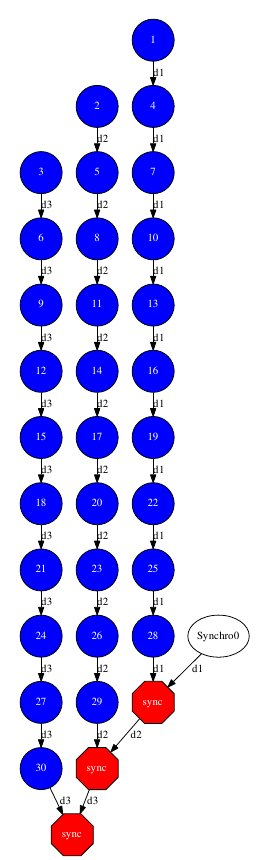
\includegraphics[width=0.3\textwidth]{./Sections/4_C/Figures/increment_graph.jpeg}
    \caption{C increment tasks graph} 
    \label{fig:increment_c}
\end{figure}

%%%%%%%%%%%%%%%
%% MATMUL
%%%%%%%%%%%%%%%
\newpage
~
%\subsection{Matmul}
